%pdflatex-this
\documentclass{beamer}

\setbeamertemplate{caption}[numbered]
%\setbeamertemplate{note page}[plain]
%\setbeameroption{show notes}
\setbeamerfont{note page}{size=\scriptsize}

\usepackage[czech]{babel}
\usepackage[utf8]{inputenc}
\usepackage{graphicx}
\usepackage{hyperref}
\usepackage{verbatim}

\newcommand{\N}[1]{\note{- #1\\}}
%\AtBeginNote{%
%	\let\enumerate\itemize%
%        \let\endenumerate\enditemize%
%}

\setlength\fboxsep{0pt}
\setlength\fboxrule{3pt}

\mode<presentation> {
	\usetheme{Boadilla}
	%\usetheme{lankton-keynote}
	%\usetheme{Berlin}
}

\author[Tomáš Kukrál]{Tomáš Kukrál}
\institute[tech@SU]{Studentská unie ČVUT - klub tech@SU}
\title[Koleje a menzy]{Koleje a menzy}
\date{11.6.2014}

\begin{document}

\begin{frame}
	\titlepage
\end{frame}

\section{Menzy}
\begin{frame}
	\begin{center}
	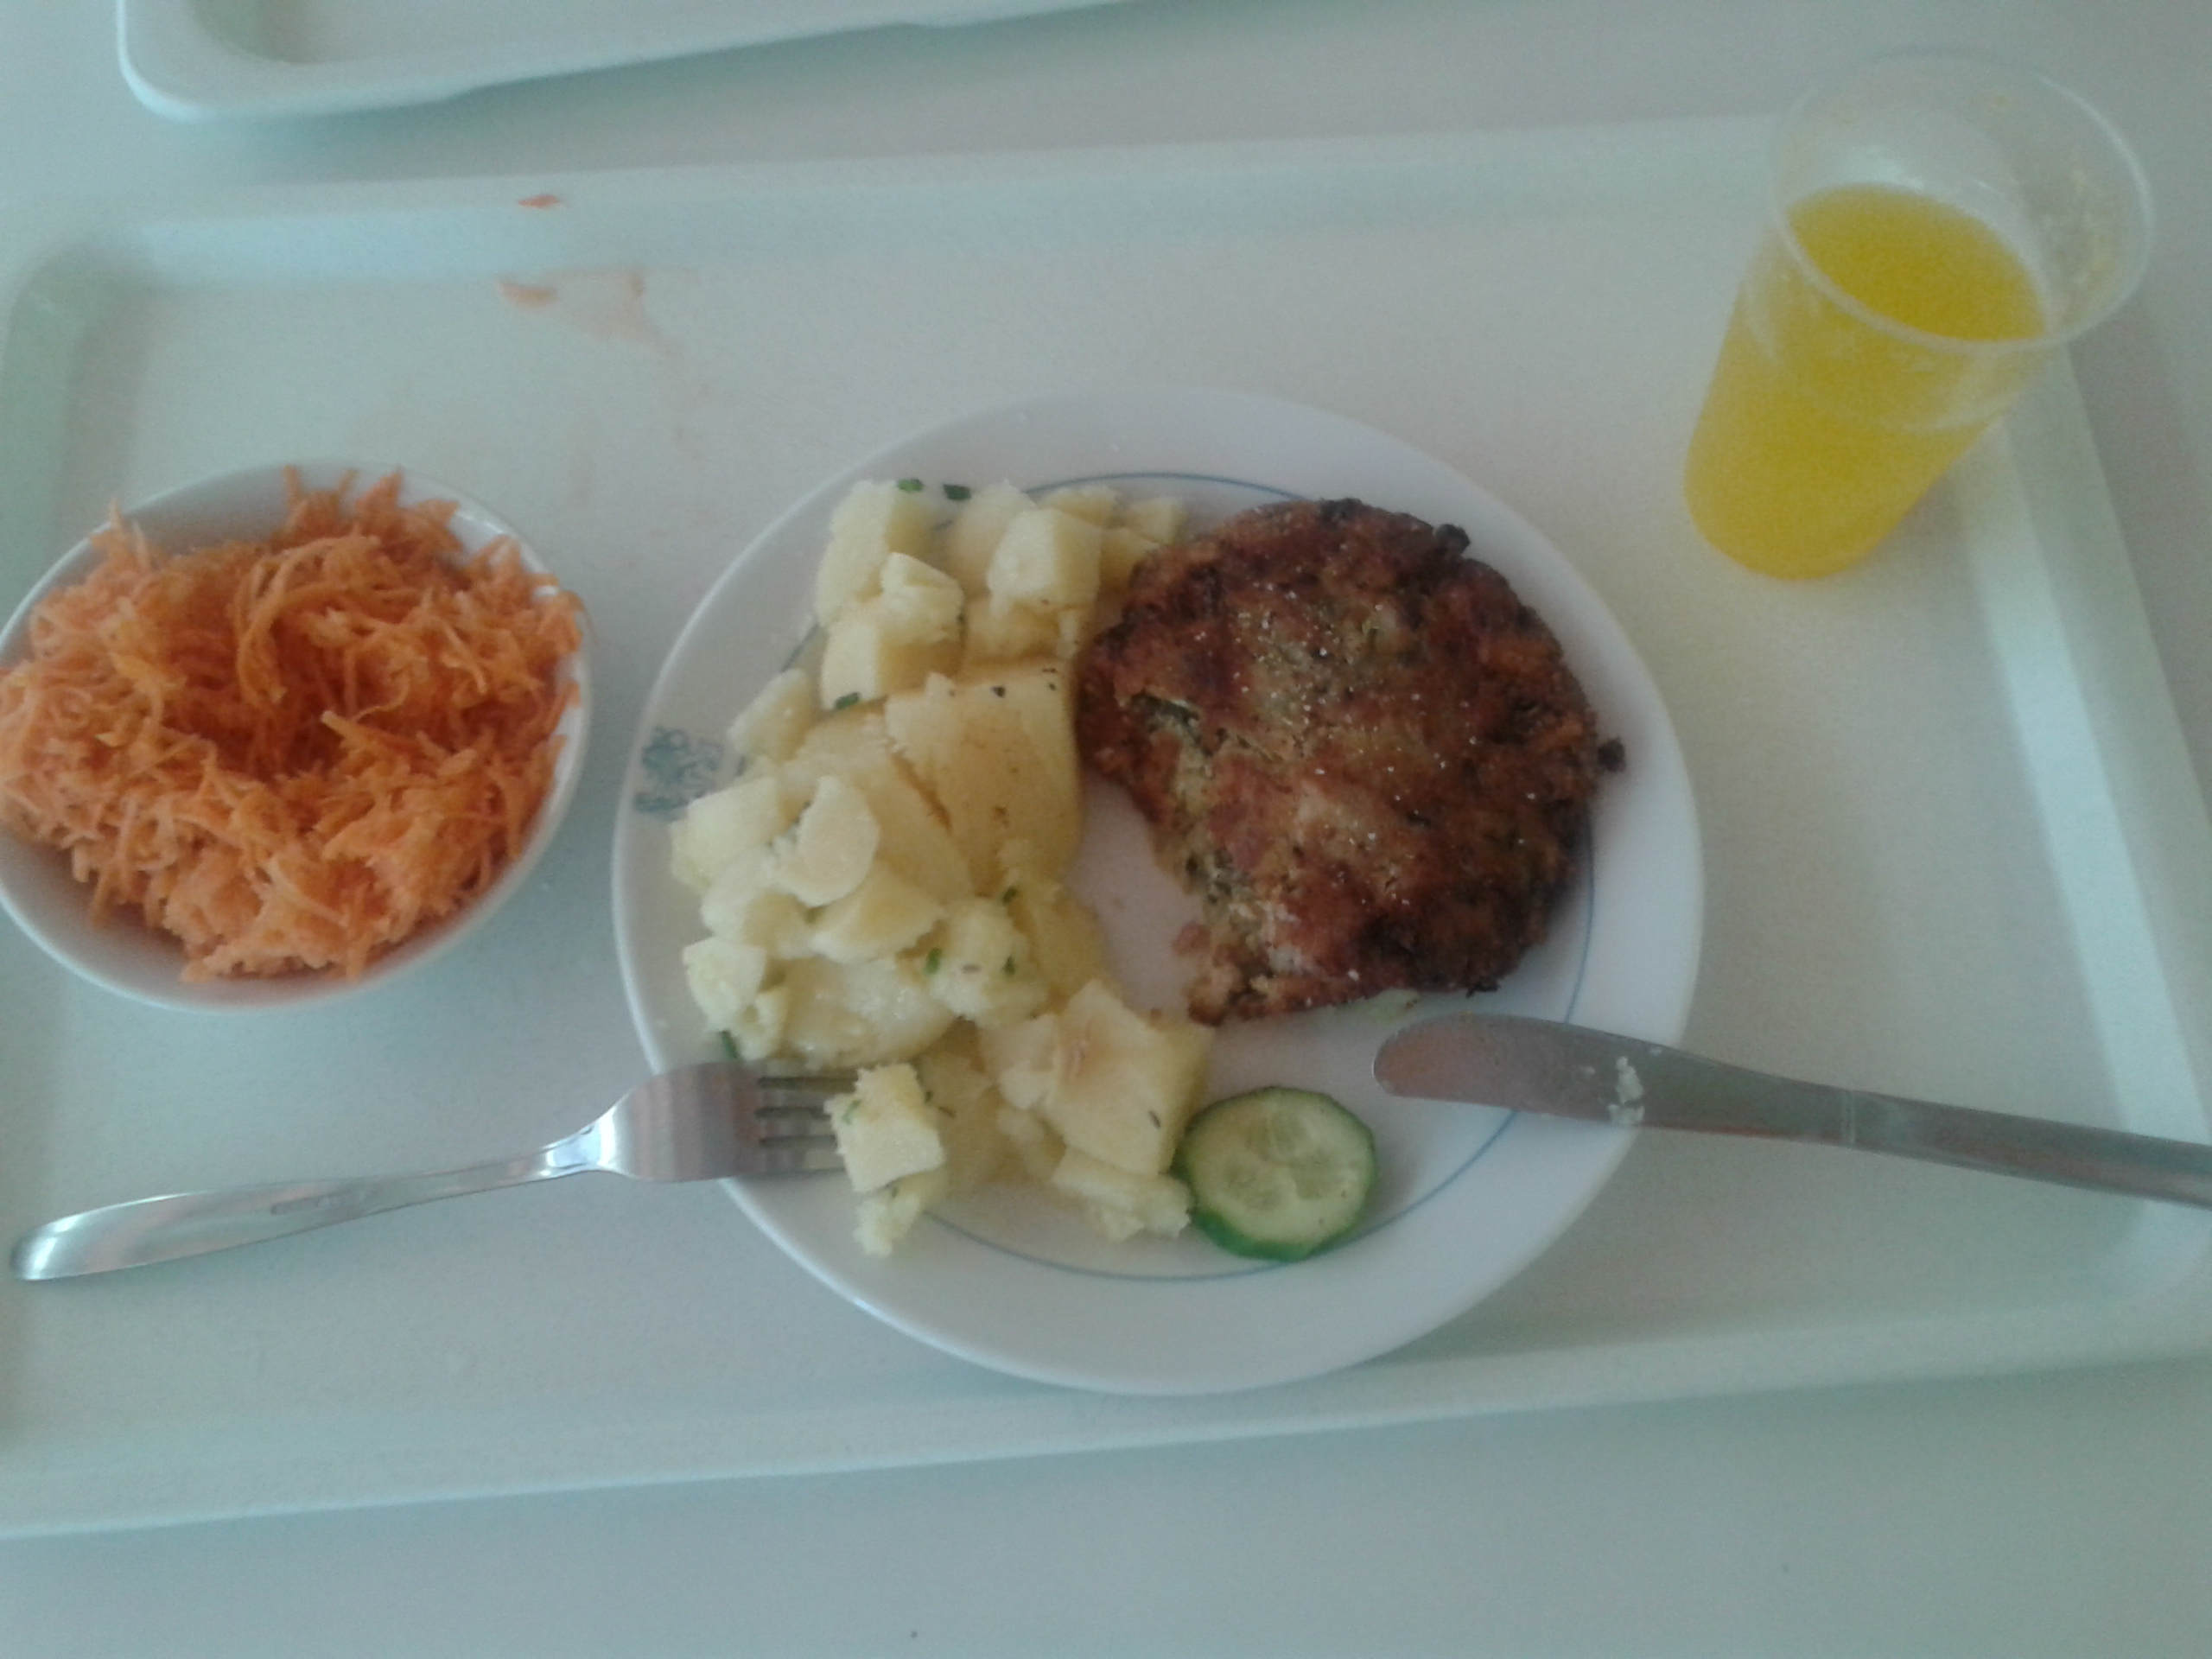
\includegraphics[width=0.9\textwidth]{obed_foto.jpg}
	\end{center}
\end{frame}

\begin{frame}
	\begin{center}
	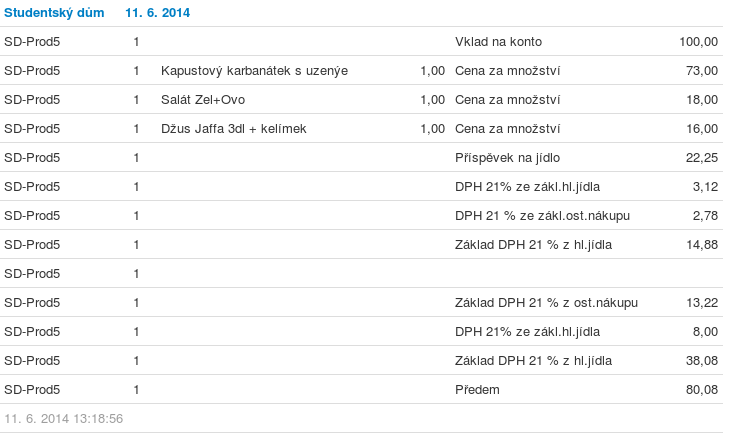
\includegraphics[width=0.9\textwidth]{obed_cena.png}
	\end{center}
\end{frame}

\begin{frame}
	\begin{center}
	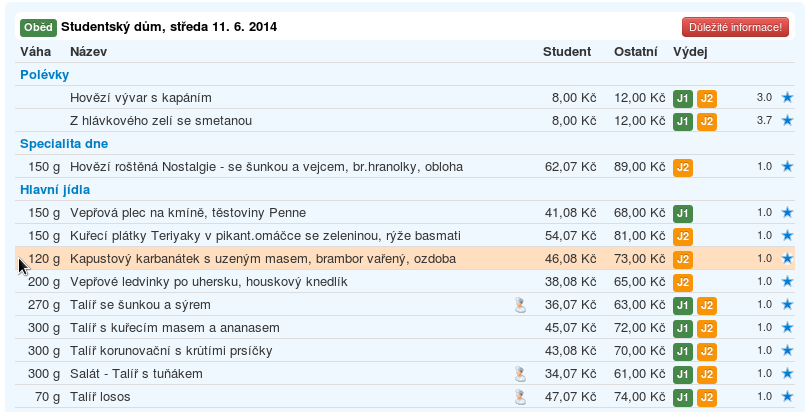
\includegraphics[width=0.9\textwidth]{obed_cenik.png}
	\end{center}
\end{frame}


\section{Koleje Strahov}
\begin{frame}{Koleje Strahov}
	\begin{columns}[c]
		\column{0.4\textwidth}
			\begin{center}
				
\includegraphics[width=0.9\textwidth]{logo_sh.png}
			\end{center}

			\begin{itemize}
				\item všichni bydlí tu
				\item 1000Mbps
				\item Středisko Unixových technologí
				\item fitcentra
				\item SHOW, OpenAir
			\end{itemize}
		\column{0.6\textwidth}
			\begin{center}
				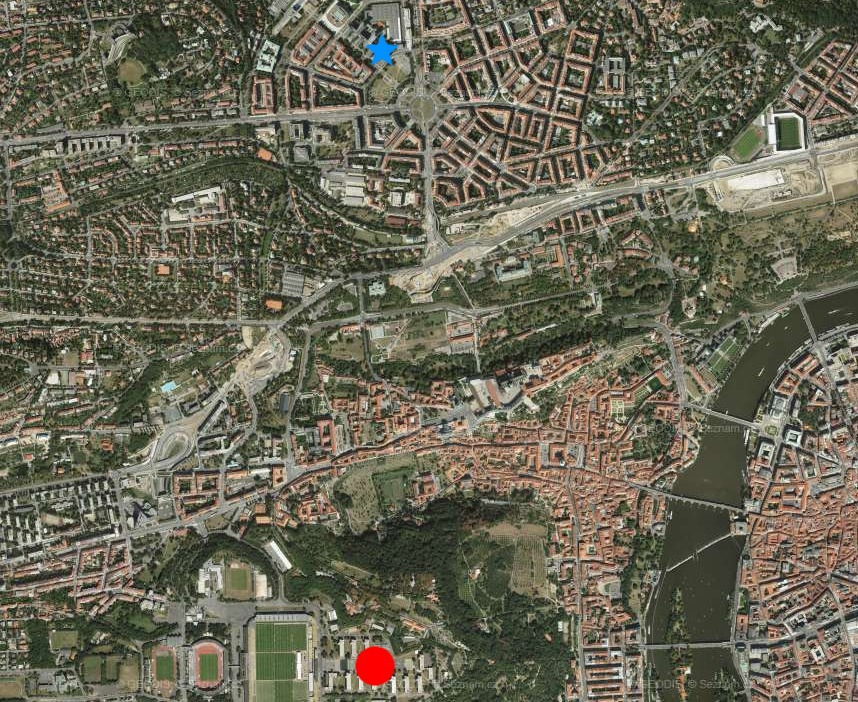
\includegraphics[width=\textwidth]{mapa_sh.png}
			\end{center}
	\end{columns}

\end{frame}


\section{Koleje Podolí}
\begin{frame}{Koleje Podolí}
	\begin{columns}[c]
		\column{0.4\textwidth}
			\begin{center}
				
\includegraphics[width=0.9\textwidth]{logo_pod.png}
			\end{center}

			\begin{itemize}
				\item posilovna
				\item boulder
				\item Mezi Bloky
			\end{itemize}
		\column{0.6\textwidth}
			\begin{center}
				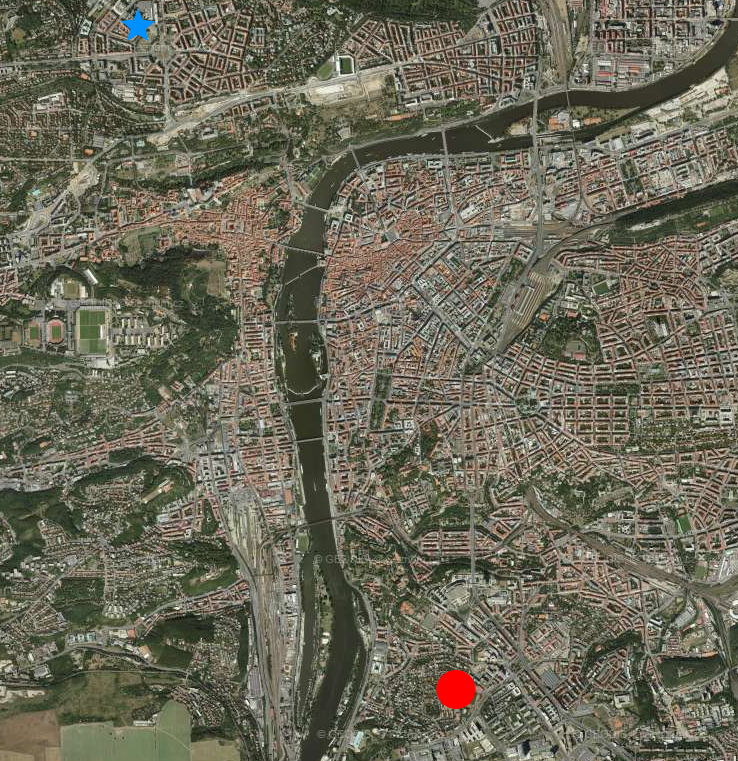
\includegraphics[width=\textwidth]{mapa_pod.png}
			\end{center}
	\end{columns}

\end{frame}

\section{Kolej Bubeneč}
\begin{frame}{Kolej Bubeneč}
	\begin{columns}[c]
		\column{0.4\textwidth}
			\begin{center}
				
\includegraphics[width=0.9\textwidth]{logo_buk.png}
			\end{center}

			\begin{itemize}
				\item Dejvice
				\item posilovna
				\item studovna Cisco akademie
				\item hřiště (SUZu)
			\end{itemize}
		\column{0.6\textwidth}
			\begin{center}
				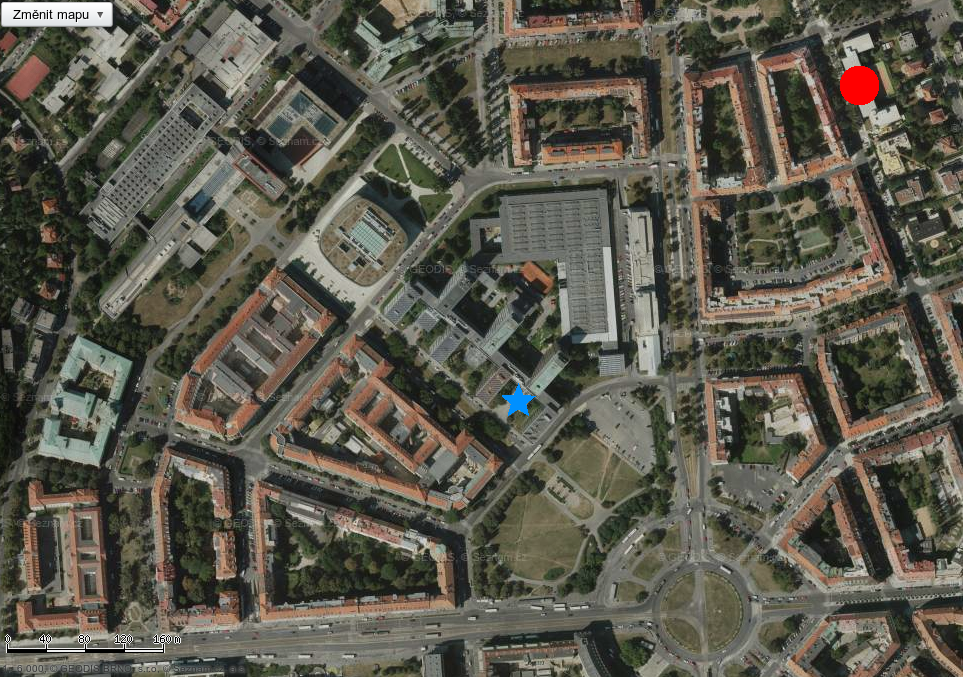
\includegraphics[width=\textwidth]{mapa_buk.png}
			\end{center}
	\end{columns}

\end{frame}

\section{Sinkuleho a Dejvická kolej}
\begin{frame}{Sinkuleho a Dejvická kolej}
	\begin{columns}[c]
		\column{0.4\textwidth}
			\begin{center}
				
\includegraphics[width=0.9\textwidth]{logo_sin.png}
			\end{center}

			\begin{itemize}
				\item Dejvice
				\item posilovna
				\item tiskárna
				\item bázen se Spidermanem
			\end{itemize}
		\column{0.6\textwidth}
			\begin{center}
				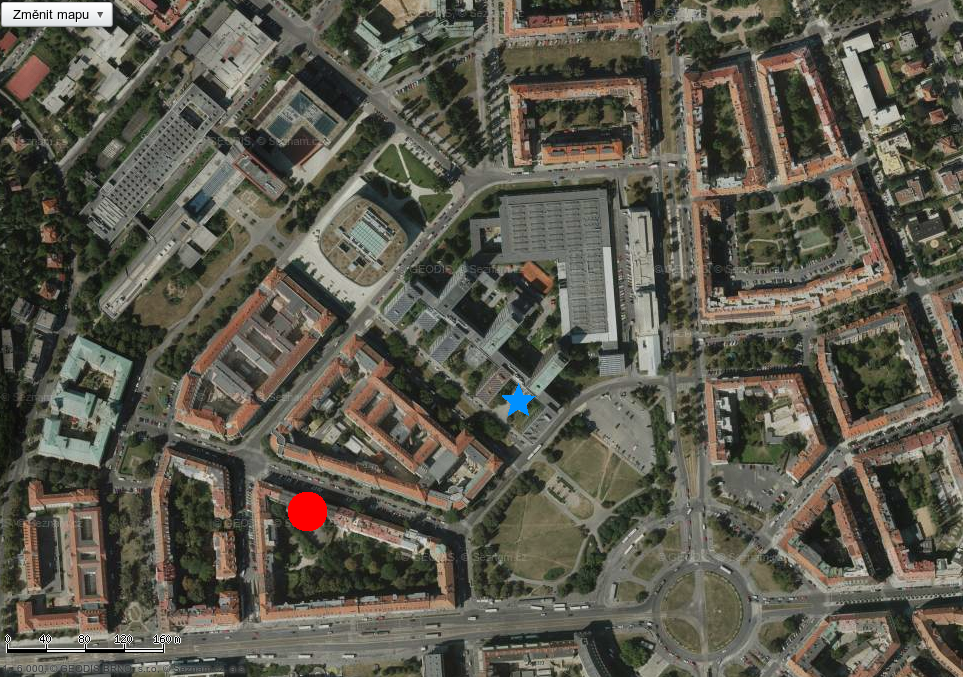
\includegraphics[width=\textwidth]{mapa_sin.png}
			\end{center}
	\end{columns}
\end{frame}


\section{Kolej Orlík}
\begin{frame}{Kolej Orlík}
	\begin{columns}[c]
		\column{0.4\textwidth}
			\begin{center}
				
\includegraphics[width=0.7\textwidth]{logo_ok.png}
			\end{center}

			\begin{itemize}
				\item Dejvice
				\item DVgrab
			\end{itemize}
		\column{0.6\textwidth}
			\begin{center}
				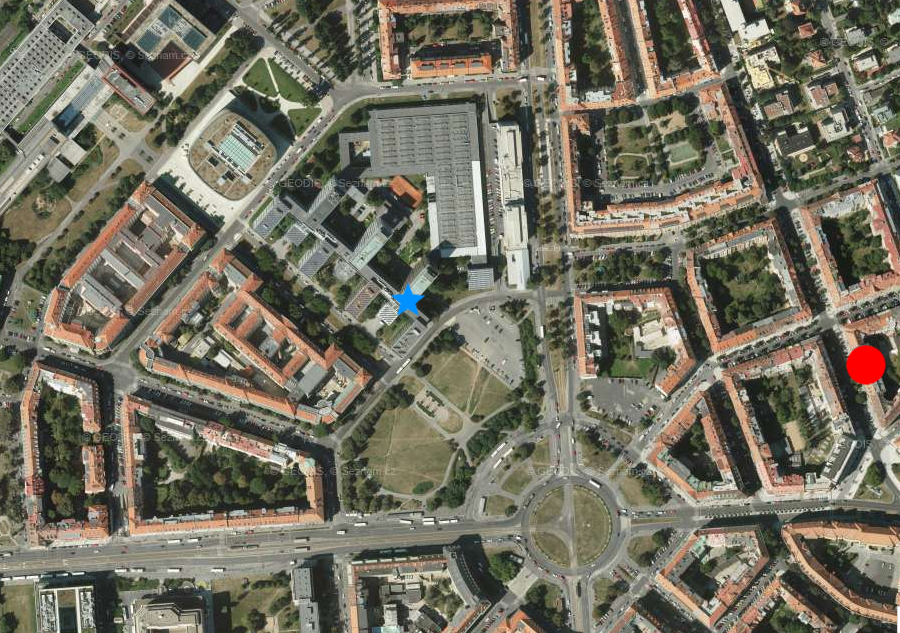
\includegraphics[width=\textwidth]{mapa_ok.png}
			\end{center}
	\end{columns}

\end{frame}

\section{Masarykova kolej}
\begin{frame}{Masarykova kolej}
	\begin{columns}[c]
		\column{0.4\textwidth}
			\begin{center}
				
\includegraphics[width=0.9\textwidth]{logo_mk.png}
			\end{center}

			\begin{itemize}
				\item Dejvice
				\item rýsovna
				\item hudebna
				\item studovny
			\end{itemize}
		\column{0.6\textwidth}
			\begin{center}
				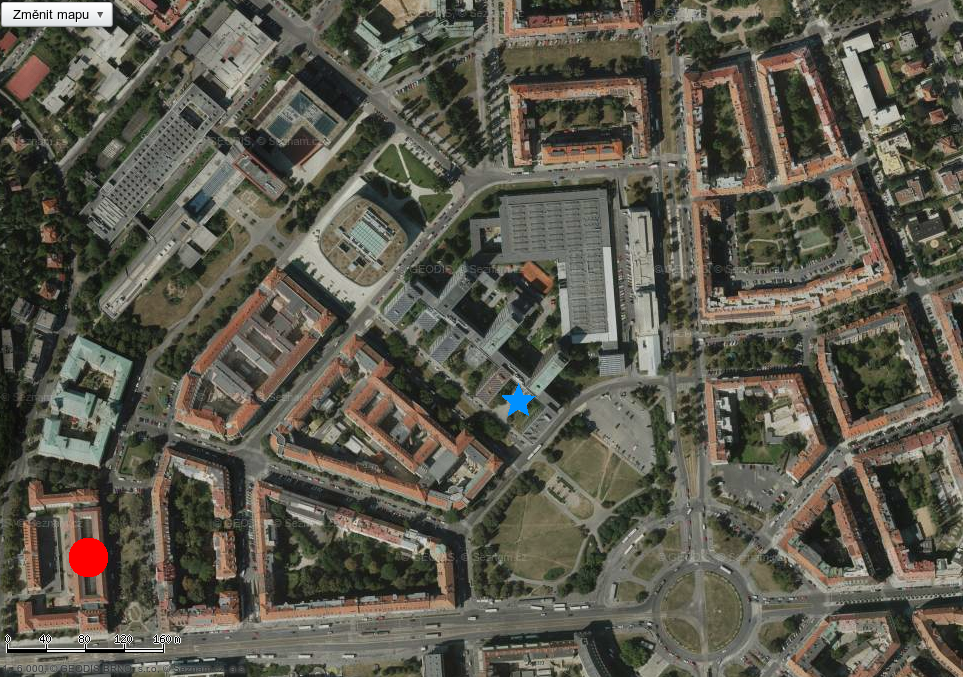
\includegraphics[width=\textwidth]{mapa_mk.png}
			\end{center}
	\end{columns}

\end{frame}

\section{Dotazy}
\begin{frame}
	\begin{center}
	Díky za pozornost,
	nějaké dotazy?
	\end{center}
\end{frame}

\end{document}
